\section{ПРАКТИЧЕСКАЯ ЧАСТЬ}


\subsection{Используемые инструменты}

\begin{itemize}
 \item Python 3


 \item NumPy


 \item Pandas


 \item Matplotlib


 \item Pymorphy2


 \item Razdel


 \item Scikit-learn


 \item TensorFlow


 \item JavaScript


 \item HTML и CSS
\end{itemize}


% \begin{itemize}
%  \item Python 3;
%  \begin{itemize}
%   \item nltk;
%   \item Pymorphy2;
%   \item NumPy;
%   \item Pandas;
%   \item Razdel;
%   \item Matplotlib;
%   \item Scikit-learn;
%   \item TensorFlow.
%  \end{itemize}
%
%  \item JavaScript;
%  \item HTML и CSS.
% \end{itemize}


\subsection{Сбор данных}


Самым главным этапом перед созданием моделей-классификаторов является сбор данных, этот процесс включает в себя несколько основных этапов:

\bigskip
\begin{itemize}
 \item обработка и подготовка текстов;
 \item разметка текстов;
 \item обработка полученных результатов.
\end{itemize}

\subsubsection{Обработка и подготовка текстов}

В качестве основного текста для разметки был взят роман Михаила Афанасьевича Булгакова <<Мастер и Маргарита>>.

\bigskip
Обработка документа:

\bigskip
\begin{enumerate}
\item произведение было очищено от нежелательных подстрок регулярными выражениями;
\item разделено на тексты по символу перевода строки <<\textbackslash n>>;
\item из полученных текстов восстановлена прямая речь;
\item тексты содержащие больше 52 слов разделены с использованием библиотеки <<razdel>>.
\end{enumerate}

\bigskip
Формирование заданий:

\bigskip
\begin{itemize}
 \item для разметки выделены тексты от 5 до 52 слов;
 \item для каждого текста определен контекст:  не менее 40 слов перед и не менее 15 после текста.
\end{itemize}



\subsubsection{Разметка текстов}

Чтобы приступить к разметке сначала нужно определить множество меток классов, для этого обратимся к истории создания эмоциональных моделей ведушими профессорами в области изучения эмоций. В 1980 году Роберт Плутчик в своей работе \cite{Plutchik} определил колесо эмоций рис. \ref{fig:plutchik}. Данная модель была взята за основу и дополнена моделью Пола Экмана, которую он описал в работе \cite{Ekman2004} 2004 года и обновил в статье \cite{Ekman2011} 2011 года.

\begin{figure}[ht]
    \centering
    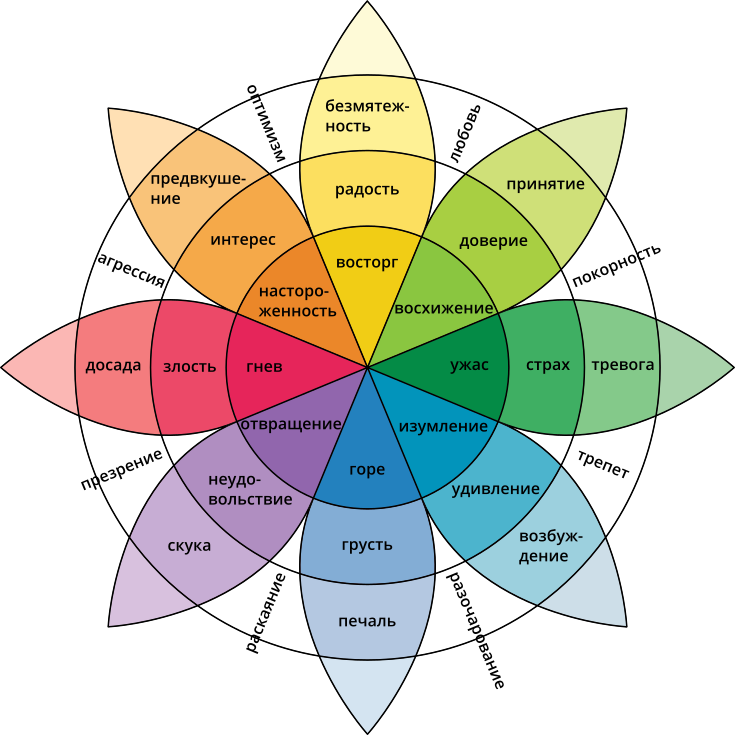
\includegraphics[scale=0.5]{plutchik.png}
    \caption{Колесо эмоции Роберта Плутчика}
    \label{fig:plutchik}
\end{figure}

В результате получилось множество, состоящее из 9 основных эмоций и их производных, дополненное нейтральным классом:

\bigskip
\begin{itemize}
\item \textbf{Злость} (anger) --- желание выразить агрессию или причинить зло, общая для обеих моделей.\\
Может проявляться в словах, мимике, поступках.
Примеры: злость на оскорбление, на несправедливость, злость на плохое отношение.\\
Гнев --- более интенсивная эмоция, досада --- менее.

\item \textbf{Интерес} (anticipation) --- предчувствие важного события, только в модели Плутчика.\\
Проявляется в нетерпении, волнении.
Примеры: ожидание праздника, ожидание начала каникул, ожидание плохой оценки.\\
Настороженность --- более интенсивная, предвкушение --- менее.

\item \textbf{Радость} (joy) --- чувство удовольствия, весёлого настроения и счастья, общая для обеих моделей.\\
Проявляется в смехе, улыбке, ласковом обращении к другим.
Примеры: радость по поводу подарка, общения с другом.\\
Восторг --- более интенсивная, безмятежность --- менее.

\item \textbf{Доверие} (trust) --- ​открытое теплое отношение к чему бы то ни было (другу/животному/миру/...), только в модели Плутчика.\\
Проявляется в уверенности в положительном исходе.
Примеры: доверие другу при встрече с неожиданностями, доверие к собаке, что не укусит, доверие к доктору, что он делает полезные вещи.\\
Восхищение --- более интенсивная, принятие --- менее.

\item \textbf{Страх} (fear) --- состояние перед реальным или предполагаемым бедствием, общая для обеих моделей.\\
Проявляется в волнении, напряжении.
Пример: страх наказания, страх проигрыша, страх попасть в аварию.\\
Ужас --- более интенсивная, тревога --- менее.

\item \textbf{Удивление} (surprise) --- эмоциональная реакция на неожиданную ситуацию, общая для обеих моделей.\\
Удивление может проявляться в хороших и плохих ситуациях.
Примеры: получил плохой отзыв на работу вместо ожидаемого хорошего, директор школы привел в класс собаку, одноклассник вырос на 10 см за лето.\\
Изумление --- более интенсивная, возбуждение --- менее.


\item \textbf{Грусть} (sadness) --- отсутствие радости,​ неудовлетворенность происходящим, отстраненность, общая для обеих моделей.\\
Проявляется в нежелании веселиться с другими, желании заботы и участия.
Примеры: мама уехала в командировку надолго, не покупают собаку или велосипед, никак не дается математика.\\
Горе --- более интенсивная, печаль --- менее.

\item \textbf{Неудовольствие} (disgust) --- эмоциональная реакция на неприятную ситуацию или объект.\\
Проявляется в неприятии человека, любых вещей, ситуаций, общая для обеих моделей.
Примеры: когда сталкиваешься с неприятным запахом, грязными вещами, плохим поведением.\\
Отвращение --- более интенсивная, скука --- менее.

\item \textbf{Презрение} (contempt) --- пренебрежительное отношение к кому-чему-нибудь морально низкому, недостойному, подлому. Презрение связано с чувством превосходства. Также оно может перейти в безразличное отношение к кому-чему-то. Только в модели Экмана.

\item \textbf{Нейтральное} (neutral) --- безэмоциональное повествование.

\end{itemize}

\bigskip
Разметка осуществлялась с помощью краудсорсинговой платформы <<Яндекс.Толока>>.

\begin{definition}
 Краудсорсинг --- это привлечение добровольцев и экспетртов для выполнения определенной работы, действующих на добровольной или комерческой основе.
\end{definition}

Для получения более точной разметки данных были использованы встроенные методы и инструменты контроля качества:

\bigskip
\begin{itemize}
 \item график времени выполнения страницы заданий рис. \ref{fig:task-time} нужен, чтобы видеть на сколько вдумчиво эксперт расставляет метки;
 \item график выполнения заданий рис. \ref{fig:task-accept} показывает сколько выполнено страниц заданий, сколько просрочено и сколько пропущено. По нему можно судить о сложности выполнения задания и использовать эту информацию в процессе формирования новых пулов заданий;
 \item сформирована система правил, которая позволяет контролировать процесс разметки в автономном режиме:
    \medskip
    \begin{itemize}
     \item Eсли пропущенных подряд страниц заданий $\geqslant 10$, то заблокировать на проекте на $2$ дня;
     \item Eсли отправленных страниц заданий $\geqslant 50$, то заблокировать на проекте на $2$ дня;
     \item Минимальное время на страницу заданий --- $250$ сек. Учитывать последних страниц заданий --- $15$. Если количество ответов $\geqslant 5$ и количество быстрых ответов $\geqslant 5$, то заблокировать на проекте на $2$ дня и т.д.
    \end{itemize}
 \item размечены контрольные задания, с их помощью можно отслеживать примерную точность (accuracy), как всего набора данных, так и набора, полученного от одного эксперта;
 \item каждое задание выполняло три различных эксперта (перекрытие x3);
 \item агрегация результатов производилась методом Дэвида-Скина. Он автоматически оценивает для каждого исполнителя $|L|^2$ параметров, где $L$ --- множество возможных различных значений для агрегации и возвращает итоговый ответ и его статистическую значимость.
\end{itemize}


\begin{figure}[ht]
    \centering
    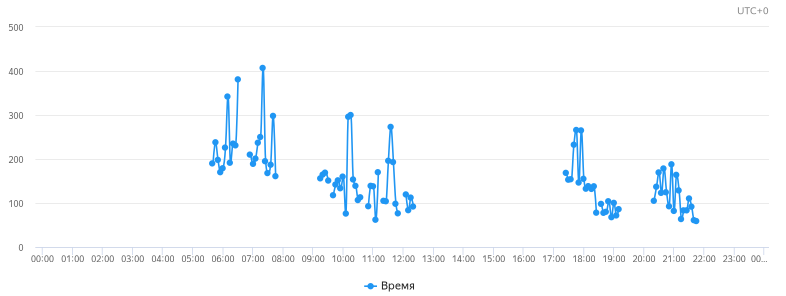
\includegraphics[scale=0.5]{task-time.png}
    \caption{Время выполнения страницы заданий (детализация по 5 минут)}
    \label{fig:task-time}
\end{figure}



\begin{figure}[ht]
    \centering
    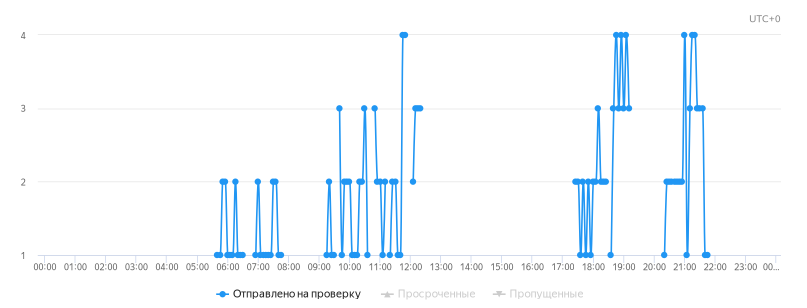
\includegraphics[scale=0.5]{task-accept.png}
    \caption{Выполнение страниц заданий (детализация по 5 минут)}
    \label{fig:task-accept}
\end{figure}

\bigskip
Была разработана форма задания рис. \ref{fig:task}. Каждое задание состоит из трех текстовых блоков. Страница заданий состоит из двух не размеченных заданий и одного контрольного, такое разбиение оптимально для получения качественных результатов. Эксперт должен прочитать каждый текстовый блок и отметить эмоции, которые, по его мнению, описаны в выделенном фрагменте.

\begin{figure}[ht]
    \centering
    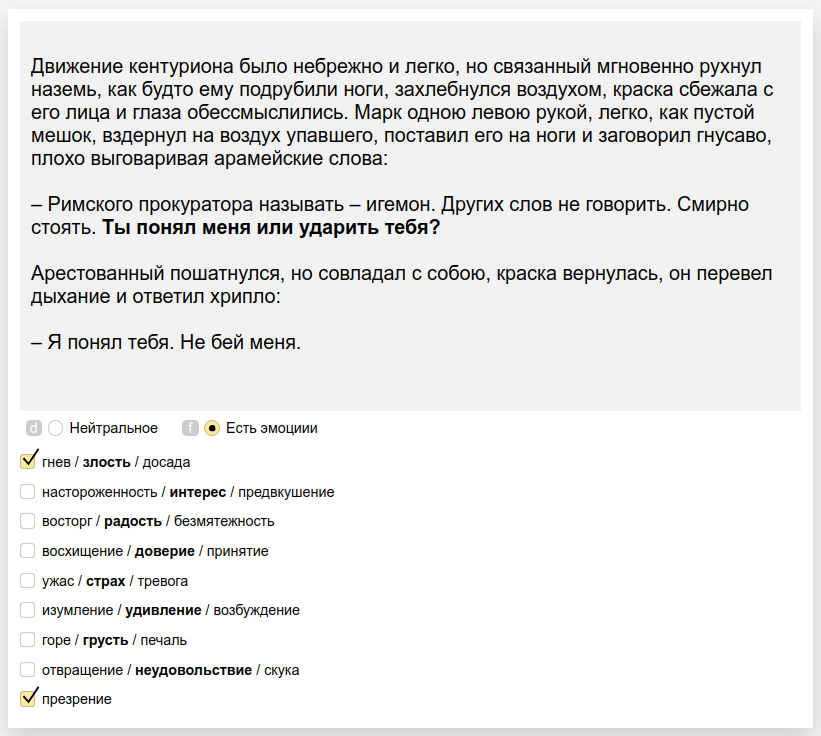
\includegraphics[scale=0.5]{task.png}
    \caption{Форма задания в сервисе <<Яндекс.Толока>>}
    \label{fig:task}
\end{figure}

\bigskip
В результате был сформирован набор данных с таким распределением классов рис. \ref{fig:class_distribution}.



\begin{figure}[ht]
    \centering
    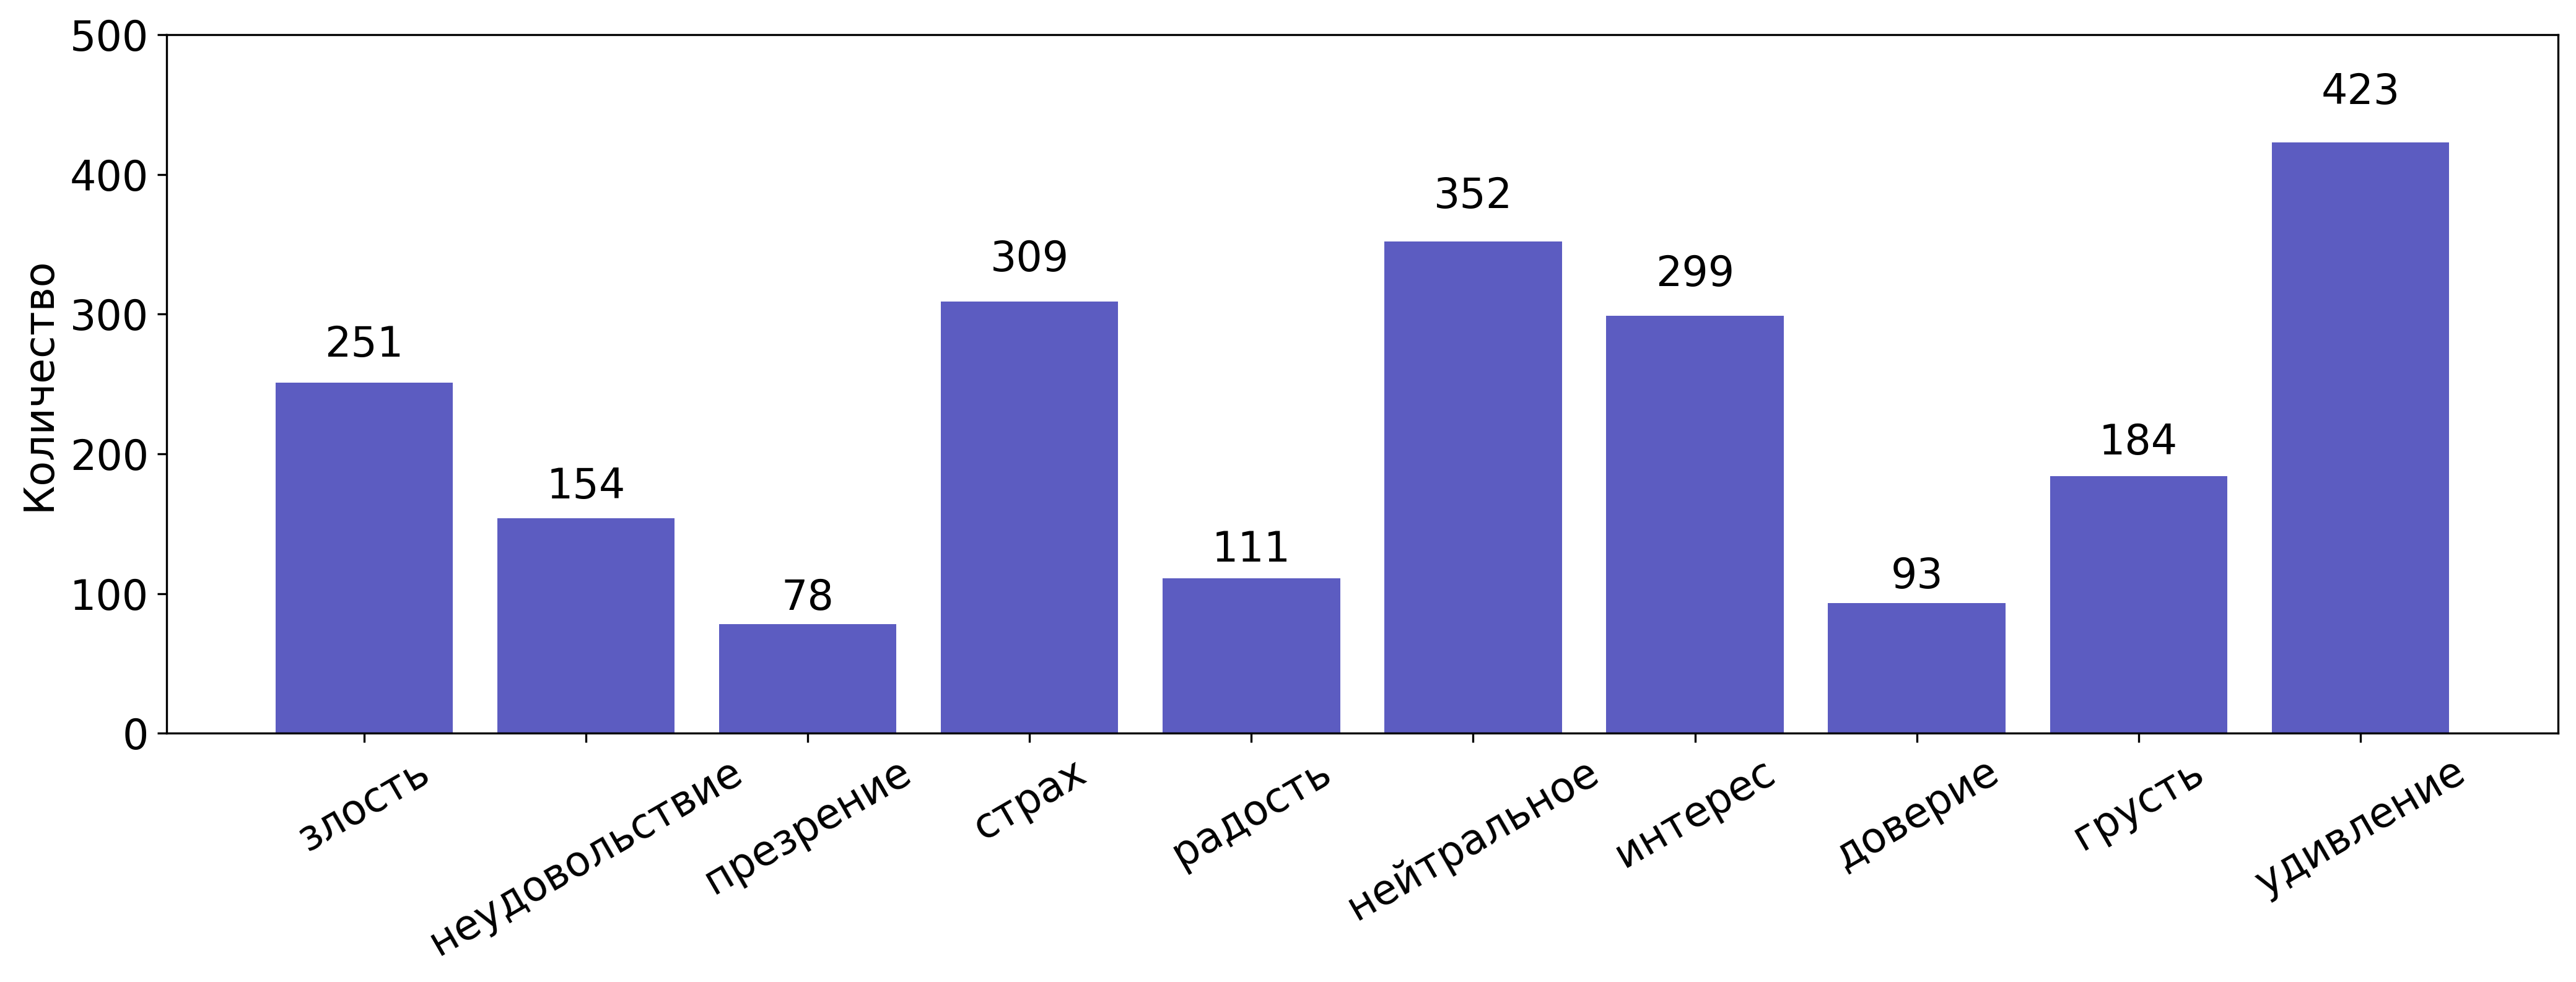
\includegraphics[scale=0.45]{class_distribution.png}
    \caption{Распределение классов в итоговом наборе данных}
    \label{fig:class_distribution}
\end{figure}

\subsection{Модели классификации}

\subsubsection{Предобработка текстов}

Чтобы работать с текстами, сначала их нужно нормализовать. Этот процесс включает несколько этапов.

\bigskip
\begin{enumerate}
 \item приводим текст к нижнему регистру;
 \item удаляем все <<не слова>> и <<стоп-слова>>;
 \item лемматизируем текст.
\end{enumerate}

\bigskip
Вот пример обработки небольшого текста:

\bigskip
\fbox{Квартира простояла пустой и запечатанной только неделю.} $\to$ \fbox{квартира простаивать пустой запечатывать неделя}


\subsubsection{Представление предложений}


Теперь текст нужно перевести в векторное пространство $R^n$, где $n$ --- размерность признаково пространства используемой модели. Пусть текст $D$ состоит из слов $d \in D$, $f$ --- модель, строящая отображение пространства слов в векторное пространство действительных чисел $f(d) \to R^n$. Тогда текст для классификатора выглядит так:

\begin{equation*}
 \frac{1}{\#D}\sum_{d \in D} f(d) \in R^n
\end{equation*}

В этой работе использованы модели предобученные на корпусе русскоязычных текстов <<Тайга>>:

\bigskip
\begin{itemize}
 \item word2vec \& skip-gram: \textit{tayga\_upos\_skipgram\_300\_2\_2019} ($n = 300$);
 \item ELMo: \textit{tayga\_lemmas\_elmo\_2048\_2019} ($n = 2048$).
\end{itemize}

\bigskip
Особенность применения ELMo заключается в том, что берется среднее значение всех слоев для каждого слова.

\subsection{Архитектура моделей классификации}

Для классификации были выбраны алгоритмы классического машинного обучения:

\bigskip
\begin{itemize}
 \item случайный лес (Random Forest);
 \item логистическая регрессия (Logistic Regression);
 \item метод опорных векторов (Support Vector Machine).
\end{itemize}

\bigskip\noindent
Схематично модели классификации представлены на рис. \ref{fig:models}.

\begin{figure}[ht]
    \centering
    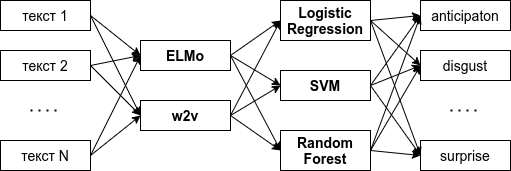
\includegraphics[scale=0.6]{models.png}
    \caption{Архитектура моделей классификации}
    \label{fig:models}
\end{figure}


\subsection{Эксперименты}

\noindent
Для эмоциональной модели Роберта Плутчика результаты получились следующие:

\bigskip
\begin{table}[ht]
\caption{Значения Macro F1 меры}
\label{tab:plutchik}
\centering
\begin{tabular}{|c|c|c|c|c|}
\hline Macro F1 & \textbf{log reg} & \textbf{SVM} & \textbf{random forest} & \textbf{tuned random forest} \\
\hline \textbf{w2v} & 0.21519548 & 0.27992996 & 0.23415391 & 0.23932876 \\
\hline \textbf{ELMO} & 0.25900211 & 0.32828541 & 0.31197309 & 0.43861588 \\
\hline
\end{tabular}
\end{table}


\noindent
Для эмоциональной модели Пола Экмана:

\bigskip
\begin{table}[ht]
\caption{Значения Macro F1 меры}
\label{tab:ekman}
\centering
\begin{tabular}{|c|c|c|c|c|}
\hline Macro F1 & \textbf{log reg} & \textbf{SVM} & \textbf{random forest} & \textbf{tuned random forest} \\
\hline \textbf{w2v} & 0.25493596 & 0.18245115 & 0.21223037 & 0.37710993 \\
\hline \textbf{ELMO}& 0.20242784 & 0.3007757 & 0.34183484 & 0.42405119 \\
\hline
\end{tabular}
\end{table}
